%%
%% This is file `sample-sigconf.tex',
%% generated with the docstrip utility.
%%
%% The original source files were:
%%
%% samples.dtx  (with options: `all,proceedings,bibtex,sigconf')
%% 
%% IMPORTANT NOTICE:
%% 
%% For the copyright see the source file.
%% 
%% Any modified versions of this file must be renamed
%% with new filenames distinct from sample-sigconf.tex.
%% 
%% For distribution of the original source see the terms
%% for copying and modification in the file samples.dtx.
%% 
%% This generated file may be distributed as long as the
%% original source files, as listed above, are part of the
%% same distribution. (The sources need not necessarily be
%% in the same archive or directory.)
%%
%%
%% Commands for TeXCount
%TC:macro \cite [option:text,text]
%TC:macro \citep [option:text,text]
%TC:macro \citet [option:text,text]
%TC:envir table 0 1
%TC:envir table* 0 1
%TC:envir tabular [ignore] word
%TC:envir displaymath 0 word
%TC:envir math 0 word
%TC:envir comment 0 0
%%
%% The first command in your LaTeX source must be the \documentclass
%% command.
%%
%% For submission and review of your manuscript please change the
%% command to \documentclass[manuscript, screen, review]{acmart}.
%%
%% When submitting camera ready or to TAPS, please change the command
%% to \documentclass[sigconf]{acmart} or whichever template is required
%% for your publication.
%%
%%
\documentclass[acmsmall]{acmart}
%%
%% \BibTeX command to typeset BibTeX logo in the docs
\AtBeginDocument{%
  \providecommand\BibTeX{{%
    Bib\TeX}}}

%% Rights management information.  This information is sent to you
%% when you complete the rights form.  These commands have SAMPLE
%% values in them; it is your responsibility as an author to replace
%% the commands and values with those provided to you when you
%% complete the rights form.
%% Camera-ready rights management (same as main paper).
\setcopyright{acmlicensed}
\copyrightyear{2026}
\acmYear{2026}
\acmJournal{PACMSE}
\acmVolume{2}                      %% TODO: verify volume from publisher
\acmNumber{FSE}                    %% TODO: verify issue from publisher
\acmArticle{0}                     %% TODO: replace with real article number from publisher
\acmMonth{7}
\acmDOI{XXXXXXX.XXXXXXX}          %% TODO: replace with real DOI from publisher rights form

\usepackage{makecell}
\usepackage{booktabs}
\usepackage{tabularx}
\usepackage{array}
\usepackage{enumitem}
%%
%% Submission ID.
%% Use this when submitting an article to a sponsored event. You'll
%% receive a unique submission ID from the organizers
%% of the event, and this ID should be used as the parameter to this command.
%%\acmSubmissionID{123-A56-BU3}

%%
%% For managing citations, it is recommended to use bibliography
%% files in BibTeX format.
%%
%% You can then either use BibTeX with the ACM-Reference-Format style,
%% or BibLaTeX with the acmnumeric or acmauthoryear sytles, that include
%% support for advanced citation of software artefact from the
%% biblatex-software package, also separately available on CTAN.
%%
%% Look at the sample-*-biblatex.tex files for templates showcasing
%% the biblatex styles.
%%

%%
%% The majority of ACM publications use numbered citations and
%% references.  The command \citestyle{authoryear} switches to the
%% "author year" style.
%%
%% If you are preparing content for an event
%% sponsored by ACM SIGGRAPH, you must use the "author year" style of
%% citations and references.
%% Uncommenting
%% the next command will enable that style.
%%\citestyle{acmauthoryear}


%%
%% end of the preamble, start of the body of the document source.
\begin{document}

%%
%% The "title" command has an optional parameter,
%% allowing the author to define a "short title" to be used in page headers.
\title{Supplementary Material: Multi-LLM Persona Generation for Virtual Focus Groups in Software Engineering: A Controlled, Multi-Domain Study of Emotional Requirements Elicitation}

%%
%% The "author" command and its associated commands are used to define
%% the authors and their affiliations.
%% Of note is the shared affiliation of the first two authors, and the
%% "authornote" and "authornotemark" commands
%% used to denote shared contribution to the research.
\author{Guangrui Fan}
\authornote{Corresponding author.}
\email{fgr@tyust.edu.cn}
\orcid{0000-0000-0000-0000}       %% TODO: replace with real ORCID
\affiliation{%
  \institution{Taiyuan University of Science and Technology}
  \city{Taiyuan}
  \country{China}
}

\author{Dandan Liu}
\email{s2134717@siswa.um.edu.my}
\orcid{0000-0000-0000-0000}       %% TODO: replace with real ORCID
\affiliation{%
  \institution{Universiti Malaya}
  \city{Kuala Lumpur}
  \country{Malaysia}
}

\author{Lihu Pan}
\email{panlh@tyust.edu.cn}
\orcid{0000-0000-0000-0000}       %% TODO: replace with real ORCID
\affiliation{%
  \institution{Taiyuan University of Science and Technology}
  \city{Taiyuan}
  \country{China}
}

\author{Rui Zhang}
\email{zhangrui@tyust.edu.cn}
\orcid{0000-0000-0000-0000}       %% TODO: replace with real ORCID
\affiliation{%
  \institution{Taiyuan University of Science and Technology}
  \city{Taiyuan}
  \country{China}
}

\author{Qian Guo}
\email{2022055@tyust.edu.cn}
\orcid{0000-0000-0000-0000}       %% TODO: replace with real ORCID
\affiliation{%
  \institution{Taiyuan University of Science and Technology}
  \city{Taiyuan}
  \country{China}
}

%%
%% By default, the full list of authors will be used in the page
%% headers. Often, this list is too long, and will overlap
%% other information printed in the page headers. This command allows
%% the author to define a more concise list
%% of authors' names for this purpose.
\renewcommand{\shortauthors}{Fan et al.}

%%
%%
%% This command processes the author and affiliation and title
%% information and builds the first part of the formatted document.
\maketitle
\clearpage
\section{Appendix}
%%
%% If your work has an appendix, this is the place to put it.
\appendix
\section{Additional results}
\begin{table}[h!]
  \centering
  \caption{Equalized-effort sensitivity (10k bootstrap replicates): median [IQR] of validated AI-only share and Jaccard overlap of validated requirement clusters between downsampled AI (2 sessions) and human baselines (EGM/FG).}
  \label{tab:equalized}
  \small
  \setlength{\tabcolsep}{5.5pt}
  \begin{tabular}{@{}lccc@{}}
    \toprule
    \textbf{Domain} & \makecell{\textbf{AI-only validated}\\\textbf{share (median [IQR])}} & \makecell{\textbf{Jaccard}\\\textbf{AI vs.\ EGM}} & \makecell{\textbf{Jaccard}\\\textbf{AI vs.\ FG}} \\
    \midrule
    A (mental health) & 46.9\% [42.3, 50.8] & 0.31 [0.27, 0.36] & 0.38 [0.33, 0.43] \\
    B (finance)       & 45.2\% [41.0, 50.1] & 0.29 [0.24, 0.34] & 0.35 [0.30, 0.41] \\
    C (fitness)       & 44.4\% [40.5, 49.5] & 0.33 [0.27, 0.37] & 0.36 [0.31, 0.42] \\
    \bottomrule
  \end{tabular}
\end{table}


\begin{table}[h!]
  \centering
  \caption{Inter-rater and coding reliability with 95\% CIs. ICC(2,$k$) for blind ratings; Krippendorff’s $\alpha$ for interaction codes.}
  \label{tab:reliability}
  \small
  \begin{tabular}{@{}l l@{}}
    \toprule
    \textbf{Measure} & \textbf{Estimate [95\% CI]} \\
    \midrule
    Relevance (ICC(2,$k$))  & 0.82 [0.77, 0.86] \\
    Clarity (ICC(2,$k$))    & 0.80 [0.74, 0.85] \\
    Feasibility (ICC(2,$k$))& 0.78 [0.70, 0.84] \\
    Innovation (ICC(2,$k$)) & 0.75 [0.68, 0.82] \\
    \midrule
    \textsc{gd-conflict} ($\alpha$)   & 0.73 [0.66, 0.80] \\
    \textsc{gd-empathy} ($\alpha$)    & 0.70 [0.61, 0.78] \\
    \textsc{gd-resolution} ($\alpha$) & 0.76 [0.69, 0.83] \\
    \bottomrule
  \end{tabular}
\end{table}

\begin{figure}[h!]
  \centering
  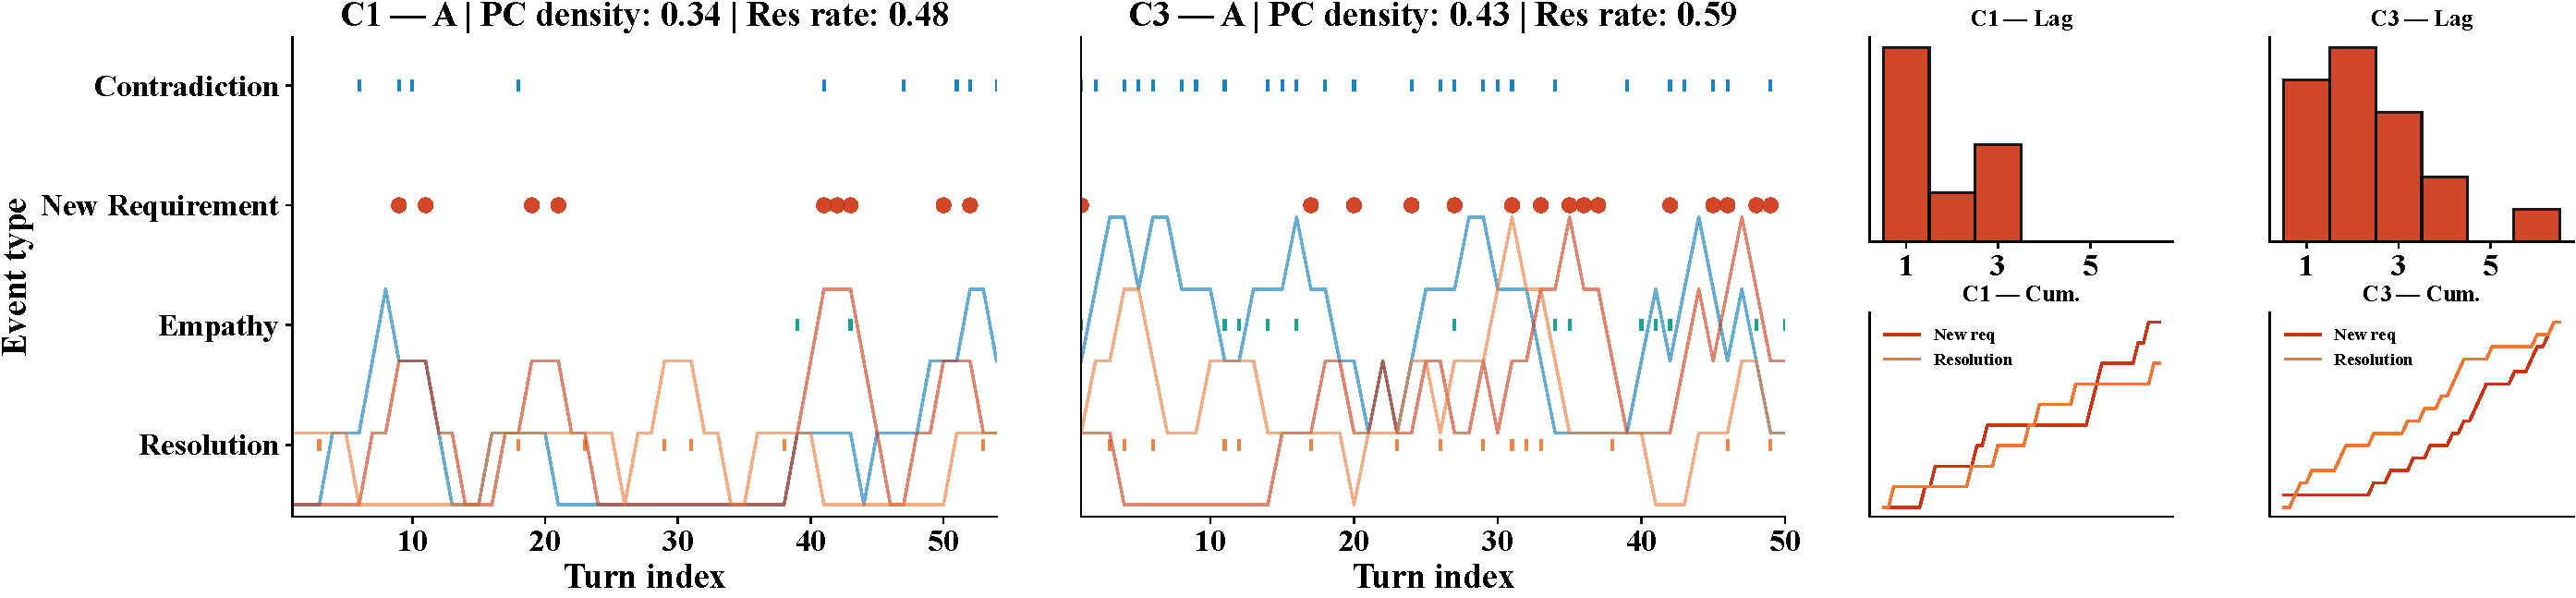
\includegraphics[width=\linewidth]{conflict_timelines_no_title.pdf}
  \caption{Event timelines and dynamics across two representative sessions (Domain~A). Left and middle panels show turn-level rasters for Contradiction, New requirement, Empathy, and Resolution, with smoothed occurrence rates. The right column summarizes per-session dynamics: top row, the first-lag from a contradiction to the subsequent new requirement; bottom row, cumulative counts of new requirements and resolutions.}
  \label{fig:conflict-timelines-supp}
\end{figure}

\begin{table}[h!]
  \centering
  \caption{Orchestration invariants and limits (all domains, all AI conditions).}
  \label{tab:orchestration-supp}
  \small
  \setlength{\tabcolsep}{6pt}
  \begin{tabular}{@{}l l@{}}
    \toprule
    \textbf{Aspect} & \textbf{Specification} \\
    \midrule
    Turn-taking & Round-robin per question; fixed persona order within question \\
    Token limits & $\leq 300$ tokens/persona/turn; $\leq 50$--$60$ total turns/session \\
    Questions & Five core surfaces; domain-specific exemplars only \\
    Challenge turns & $\leq 2$ per session; trigger after Q2 if conflict is weak \\
    Context window & Full history; summarize earliest turns if $>85\%$ window \\
    Persona--model mapping & Persona voiced by its creator model (C2/C3); single model in C0/C1 \\
    Role integrity & Speaker tags; role-break detector; single retry; both attempts logged \\
    Safety refusals & Single retry under identical parameters; refusal recorded if persistent \\
    Moderator probes & Standardized, non-leading probes \\
    Logging & Per-turn tokens/latency/flags; model/version strings; seeds or proxies \\
    \bottomrule
  \end{tabular}
\end{table}

\section{Protocol Invariants and Interview Stimuli}

\begin{table}[h!]
  \centering
  \caption{Checklist of protocol elements: invariant vs.\ domain-adapted.}
  \label{tab:invariants-vs-adapted}
  \small
  \begin{tabular}{@{}p{2.8cm} p{5.5cm} p{5.8cm}@{}}
    \toprule
    \textbf{Protocol element} & \textbf{Invariant (fixed)} & \textbf{Domain-adapted (templated)} \\
    \midrule
    Persona pipeline (C1--C3) & 3-step procedure; decoding params; retry policy & \texttt{[DOMAIN]}, \texttt{[CONTEXTS]}, \texttt{[SENSITIVE ASPECTS]} \\
    Orchestration & Round-robin, token limits, challenge-turn cap, context policy & Exemplars inside the five question surfaces only \\
    Instruments & Rating scales (1--5), anchors, bias guardrails & One illustrative example per domain (appendix) \\
    Coding rubrics & ER/GD codebooks; conflict typology; persona attributes & None (definitions constant) \\
    Validation rules & Blind cross-rating; threshold rule; QC & One-paragraph domain brief before blocks \\
    Bias audit & Guardrails; audit procedure & 2--3 domain red-flag terms (appendix) \\
    EGM procedure & Four-step flow; tracing; prioritization rubric & 3--5 example cards; same base deck \\
    Human baselines & Moderator script; session length; transcription & Domain vignettes in icebreaker only \\
    Reflective interviews & Source-blind first pass; reveal script; semi-structured guide & Stimuli mix balanced by domain; neutral domain brief \\
    \bottomrule
  \end{tabular}
\end{table}

\begin{table}[h!]
  \centering
  \caption{Stimuli composition and quotas per reflective interview.}
  \label{tab:stimuli-mix}
  \small
  \begin{tabular}{@{}lccc@{}}
    \toprule
    \textbf{Stimulus type} & \textbf{Quota} & \textbf{Source balance} & \textbf{Notes} \\
    \midrule
    High-scoring items     & 4--5  & Mix AI / Human (incl.\ EGM) & Highest median relevance/innovation \\
    Unique-source items    & 3--4  & At least 2 AI-only; 1 EGM-only & Validated or near-threshold \\
    Contrast pairs         & 2--3 pairs & AI vs.\ EGM/Human & Same need, divergent solution \\
    \bottomrule
  \end{tabular}
\end{table}

\section{Baseline Mapping and Prior-Work Comparison}
\label{sec:supp-baseline-mapping}
This appendix provides two small ``navigation'' tables to help readers (i) map our conditions to baseline patterns commonly used in LLM‑persona pipelines and (ii) situate this paper relative to representative prior lines of work. The comparison is intended to be informative rather than exhaustive.

\begin{table}[h!]
  \centering
  \caption{Mapping common baseline patterns to our experimental conditions.}
  \label{tab:baseline-mapping}
  \small
  \setlength{\tabcolsep}{5pt}
  \begin{tabularx}{\linewidth}{@{}p{3.25cm}X p{2.8cm}@{}}
    \toprule
    \textbf{Baseline pattern} & \textbf{Description (typical)} & \textbf{Condition(s) here} \\
    \midrule
    Single‑model one‑shot personas & Generate \(K\) personas in one pass; no workflow iteration. & C0 \\
    Single‑model iterative refinement & Expand/refine personas over multiple steps with a fixed workflow. & C1 \\
    Same‑model multi‑voice roleplay & Multiple persona voices produced by the same base model (prompt‑diverse role priors) to test ``multi‑voice'' structure without provider heterogeneity. & C1‑MV \\
    Multi‑model sequential persona generation & Different models contribute personas across steps; creator–voice mapping preserved to keep heterogeneous voices stable in dialog. & C2, C3 \\
    Multi‑model dialogic focus group & Moderated multi‑party dialog among heterogeneous persona voices, followed by extraction/deduplication and validation. & C3 \\
    Same‑model multi‑step (ablation) & Multi‑step pipeline but all steps voiced by the same model to isolate plurality \emph{structure} from provider capability. & C3‑SM \\
    \bottomrule
  \end{tabularx}
\end{table}

\begin{table}[h!]
  \centering
  \caption{Feature coverage compared to representative prior work (as reported). ``Blind validation'' denotes independent, source‑blinded human ratings of outputs; ``Baselines'' denotes comparison against human focus groups and/or EGM.}
  \label{tab:priorwork-compare}
  \scriptsize
  \setlength{\tabcolsep}{3.5pt}
  \begin{tabular}{@{}p{3.5cm}cccccc@{}}
    \toprule
    \textbf{Work / line of work} & \textbf{Multi‑model} & \textbf{Dialogic} & \textbf{Blind} & \textbf{Baselines} & \textbf{Cross‑domain} & \textbf{Mechanisms} \\
    \midrule
    \textbf{This work} (multi‑LLM personas + simulated focus groups for ER elicitation) & Yes & Yes & Yes & Yes (FG+EGM) & Yes & Yes (conflict/empathy) \\
    Lazik et al.\ (RE'25; diversity aspects in LLM‑generated personas) & No & No & No & No & No & No \\
    Focus Agent (IVA'24; LLM‑powered virtual focus group) & No & Yes & No & Human FG only & No & No \\
    PersonaFlow (CHI'25; LLM‑simulated expert personas for ideation) & Not reported & Yes & No & No & No & No \\
    Wu et al.\ (EMNLP'25; personas for emotional support dialogues) & No & Yes & Not reported & No & No & No \\
    \bottomrule
  \end{tabular}
\end{table}
\section{Prompt Logs and Instructions}


\subsection{Persona Generation Prompts}

\noindent\textbf{Initial Persona Generation Prompt (Single-Model Case)}\\
\underline{Prompt Text}: 
\begin{quote}
\emph{``You are an AI assistant helping to design a mental health journaling application. 
Please generate 6 distinct user personas, each with a unique demographic profile, primary emotional triggers, motivations, and journaling usage patterns. 
Focus on aspects relevant to mental health and emotional well-being, such as stressors, anxieties, or self-improvement goals. 
Ensure each persona is coherent and detailed enough to suggest plausible user behaviors.''}
\end{quote}

We issued this single prompt to each LLM (GPT-4o, Claude 3.5, Llama-2) independently, with no follow-up interactions. 
Where possible, we configured the temperature parameter to 0.7 and limited the maximum token length to 750 tokens, to encourage moderate creativity while avoiding excessively long outputs. 
If an LLM produced truncated or incomplete personas, we prompted once more with \emph{``Please continue.''}, preserving the same temperature and max token settings.

\subsection{Two-Model Pair Generation Prompts}

For the two-model pair setups, we used a sequential prompt handoff protocol:

\noindent\textbf{Model A’s Persona Draft Prompt:}
\begin{quote}
\emph{``Generate 3 distinct user personas for a mental health journaling app, focusing on diverse emotional backgrounds, 
demographics, and journaling needs. 
Please label them as Persona A1, A2, A3, ensuring each has unique stressors, motivations, and usage habits.''}
\end{quote}

After Model A output three personas, we copied the raw text verbatim into Model B’s prompt:

\noindent\textbf{Model B's Refinement and Extension Prompt:}
\begin{quote}
\emph{``Below are 3 initial personas created by another AI. 
Please refine or expand these if needed for coherence or variety, 
and then add 3 new personas (labeled B1, B2, B3) with distinct emotional triggers and usage patterns. 
Aim for diversity in demographic traits and mental health contexts. 
The existing personas are:
[PASTE MODEL A OUTPUT HERE]
Now produce 6 final personas total.''}
\end{quote}

We recorded the exact outputs for \emph{Personas (A1, A2, A3, B1, B2, B3)}, noting any modifications made by Model B to A's initial content. 
All prompts used the same temperature (0.7) and max tokens (750) to maintain consistency.

\subsection{C3 Three-Model Sequential Prompts} 

For the triple-model sequence (C3), each model contributed two personas in turn:

\noindent\textbf{Model A (Step 1):}
\begin{quote}
\emph{``Generate 2 user personas (labeled A1, A2) for a mental health journaling application, focusing on diverse emotional profiles and daily usage patterns. 
They should have coherent backgrounds, clear emotional triggers, and plausible motivations.''}
\end{quote}

\noindent\textbf{Model B (Step 2):}
\begin{quote}
\emph{``Below are 2 personas from another model. Please refine them if needed to improve coherence or emotional variety, 
then add 2 new personas (labeled B1, B2) with distinct backgrounds and mental health triggers. 
All 4 should be consistent as a cohesive set.
Existing personas:
[PASTE MODEL A OUTPUT HERE]
Now produce a set of 4 final personas total.''}
\end{quote}

\noindent\textbf{Model C (Step 3):}
\begin{quote}
\emph{``You have 4 personas so far, from two other models. 
Please finalize them if coherence issues remain, then add 2 new personas (labeled C1, C2). 
Ensure the overall set of 6 remains demographically diverse and includes varied mental health concerns. 
The final group should be:
[PASTE Model B's 4-Persona Output Here]
''}
\end{quote}

Again, we enforced the same temperature/max tokens for each step, ensuring that Model C had access to the combined persona content from Models A and B.


\section{Moderator Scripts}

We employed a consistent moderation guide to ensure comparability between the AI-simulated focus groups and the real human focus group. Below, we outline the precise scripts and prompts used by our moderator in both contexts, along with any pre-defined probing or follow-up strategies to maintain uniformity.

\subsection{Unified Structure of Sessions}

All sessions (AI-based and human) adhered to the same core topics:
\begin{enumerate}
    \item Emotional Goals and Motivations
    \item Privacy and Trust Concerns
    \item Reactions to Automated Reminders
    \item App Features to Reduce Stress or Anxiety
    \item Potential Role of Community Support
\end{enumerate}

Each session opened with a greeting and an overview of the study’s purpose, followed by the same sequence of questions. We also ensured that any probing or follow-up questions remained as consistent as possible across AI and human sessions, so as to limit confounding factors.

\subsection{Script for the AI-Based Focus Groups}

\noindent
\textbf{Moderator Opening Statement:}
\begin{quote}
\emph{``Hello, everyone. Thank you for joining this virtual focus group about using a digital journaling app to support mental health. 
I will be asking a series of questions about your goals, concerns, and preferences. 
Please respond in character, as your assigned persona, and feel free to offer your honest perspectives on what would help or hinder your engagement with the app. 
I might ask some follow-up questions for clarity, but the main topics are standardized.''}
\end{quote}

\noindent
\textbf{Primary Questions:}
\begin{enumerate}
    \item \emph{``What emotional goals or benefits do you seek from a digital journaling app?''}
    \item \emph{``Which privacy or trust concerns come to mind when sharing personal reflections?''}
    \item \emph{``How do you feel about receiving automated reminders or prompts to journal daily?''}
    \item \emph{``Which features or design elements might reduce stress or anxiety around journaling?''}
    \item \emph{``Could community or peer support play a role in maintaining motivation?''}
\end{enumerate}

\noindent
\textbf{Probing Guidelines for AI Sessions:}
\begin{itemize}
    \item If a persona response was too vague or overly brief, the moderator used a neutral probe such as: 
    \emph{``Could you elaborate on that point?''} or \emph{``How might that affect your daily usage?''}
    \item In the event of repetition (where multiple personas restated the same idea), the moderator asked: 
    \emph{``Does anyone have a different perspective or a conflicting concern?''}
    \item If the AI drifted off-topic or defaulted to polite agreement, the moderator intervened with: 
    \emph{``Could you address a specific emotional scenario you have encountered?''}
\end{itemize}

\subsection{Script for the Human Focus Group}

\noindent
\textbf{Moderator Opening Statement:}
\begin{quote}
\emph{``Hello, everyone, and welcome. We appreciate your participation in this discussion on digital journaling for mental health. 
Our goal is to understand your emotional needs, privacy worries, and feature preferences, so that we can design an app that meets real user expectations. 
I will ask questions in a structured sequence, but please feel free to share experiences or ideas that come to mind. 
There are no right or wrong answers—your perspectives are all equally valuable.''}
\end{quote}

\noindent
\textbf{Main Discussion Questions:}
\begin{enumerate}
    \item \emph{``What emotional benefits do you hope to gain from a journaling app, and why might these be important to you?''}
    \item \emph{``Do you have any privacy or trust concerns about storing personal thoughts digitally? What would alleviate those worries?''}
    \item \emph{``How do you feel about receiving automated reminders? Would that motivate you or cause anxiety/guilt?''}
    \item \emph{``Are there particular features—such as guided prompts, mood tracking, or notifications—that could reduce frustration or stress?''}
    \item \emph{``Can a sense of community or peer support enhance your motivation to continue journaling? Why or why not?''}
\end{enumerate}

\noindent
\textbf{Probing Guidelines for Human Sessions:}
\begin{itemize}
    \item If participants gave very short answers, the moderator prompted: 
    \emph{``Could you share an example or personal anecdote that illustrates your concern?''}
    \item When participants offered contrasting views, the moderator asked others: 
    \emph{``Does anyone else have a similar or opposing feeling about that point?''}
    \item If a discussion veered off-topic, the moderator briefly acknowledged the point and redirected: 
    \emph{``That’s interesting. Let’s circle back to how it connects with the emotional goals of journaling…''}
\end{itemize}

\section{Guardrails, Retry Policy, and Summarization Prompts}

\subsection{System Guardrails (applied in all conditions)}
\noindent\textbf{System Prompt (verbatim;}
\begin{quote}\small
You are a neutral, non-judgmental facilitator assisting with \texttt{[DOMAIN]} design. 
\textbf{Do not} attribute fixed traits to protected classes or essentialize identity.
Avoid stigma and stereotypes. Prefer situational explanations over personal flaws.
Write in plain, respectful language. If a suggestion could increase harm, add a brief safety/consent note.
When stating concerns, ground them in context rather than identity. 
When proposing features, include opt-in, consent, and visibility controls if relevant (privacy-by-default).
\end{quote}

\subsection{Role-Integrity and Retry Policy}
\begin{itemize}[leftmargin=1.2em]
  \item \textbf{Speaker integrity:} Each turn is prefixed with the persona tag (e.g., \texttt{[P3]}). If the model emits a mismatched or moderator tag, we flag a role-break and \emph{regenerate that turn once} under identical parameters.
  \item \textbf{Safety refusal:} If a provider refuses, we issue a \emph{single retry} with the same prompt. Persistent refusals are recorded and the session proceeds.
\end{itemize}

\subsection{Context-Window Summarization Prompt}
\noindent\textbf{Summarizer Prompt (model-agnostic):}
\begin{quote}\small
Summarize the \textbf{earliest} block of dialogue into a concise, neutral digest that preserves distinct viewpoints, points of disagreement, and any concrete feature proposals. 
Use bullet points. Do not invent content. Return only the digest.
\end{quote}

\section{Domain-Templated Prompts}

\subsection{Generic Template (placeholders)}
\begin{quote}\small
You are assisting with \texttt{[DOMAIN]}. Generate \texttt{[K]} distinct personas with diverse demographics, emotional triggers, and usage patterns in \texttt{[TYPICAL CONTEXTS]}. 
Emphasize \texttt{[SENSITIVE ASPECTS]}. Each persona includes: brief bio; emotional triggers; motivations; boundaries; a short first-person voice snippet.
\end{quote}

\subsection{Finance / Budgeting (instantiated)}
\begin{quote}\small
[DOMAIN]=personal finance/budgeting; [K]=6; [TYPICAL CONTEXTS]=tracking spending, setting saving goals, connecting bank accounts; 
[SENSITIVE ASPECTS]=money anxiety/guilt, trust in aggregation, consent for data sharing.
\end{quote}

\subsection{Fitness / Habit Tracking (instantiated)}
\begin{quote}\small
[DOMAIN]=fitness/habit tracking; [K]=6; [TYPICAL CONTEXTS]=logging activity, streaks, social leaderboards; 
[SENSITIVE ASPECTS]=guilt after lapses, social-comparison pressure, visibility/consent.
\end{quote}


\section{Blinding Check and Rater Quality Control}

\begin{table}[h!]
  \centering
  \caption{Blinding check: source-guess accuracy (chance = 33\% with three source categories). Values are \% correct [95\% CI].}
  \label{tab:blinding}
  \small
  \begin{tabular}{@{}lccc@{}}
    \toprule
    \textbf{Domain} & \textbf{AI (C3)} & \textbf{EGM} & \textbf{Human FG} \\
    \midrule
    A (mental health) & 36\% [31, 41] & 34\% [29, 39] & 35\% [30, 40] \\
    B (finance)       & 35\% [30, 41] & 35\% [30, 40] & 36\% [31, 41] \\
    C (fitness)       & 37\% [32, 42] & 35\% [30, 40] & 34\% [29, 39] \\
    \bottomrule
  \end{tabular}
\end{table}

\begin{table}[h!]
  \centering
  \caption{Rater QC: attention checks and exclusions.}
  \label{tab:raterqc}
  \small
  \begin{tabular}{@{}l l@{}}
    \toprule
    \textbf{QC Metric} & \textbf{Value} \\
    \midrule
    Raters enrolled & 24 \\
    Raters excluded (failed $\geq$2 of 4 attention checks) & 2 \\
    Ratings dropped (min-time violations) & 4.8\% \\
    Items removed due to QC & 0 \\
    \bottomrule
  \end{tabular}
\end{table}


\section{Validation-Rule Sensitivity Analyses}

\begin{table}[h!]
  \centering
  \caption{Stricter validation thresholds for AI-only items (session-averaged; mean$\pm$SD). Baseline rule: median relevance $\ge 4$ or $\ge 60\%$ of raters $\ge 4$.}
  \label{tab:val-threshold}
  \small
  \begin{tabular}{@{}l l c c c@{}}
    \toprule
    \textbf{Domain} & \textbf{Condition} & \textbf{Baseline} & \textbf{Median $\ge$ 4.5} & \textbf{Rel. $\ge$4 \& Clar. $\ge$4} \\
    \midrule
    A & C1 & $36.6\%\pm5.5\%$ & $30.2\%\pm4.8\%$ & $28.3\%\pm4.6\%$ \\
      & C3 & $53.6\%\pm2.3\%$ & $44.1\%\pm3.7\%$ & $42.0\%\pm3.5\%$ \\
    \midrule
    B & C1 & $39.9\%\pm1.5\%$ & $33.3\%\pm2.0\%$ & $31.0\%\pm2.2\%$ \\
      & C3 & $52.0\%\pm5.5\%$ & $44.6\%\pm4.6\%$ & $42.1\%\pm4.4\%$ \\
    \midrule
    C & C1 & $36.6\%\pm2.0\%$ & $29.8\%\pm2.5\%$ & $27.8\%\pm2.6\%$ \\
      & C3 & $51.0\%\pm2.9\%$ & $43.2\%\pm3.2\%$ & $41.0\%\pm3.3\%$ \\
    \bottomrule
  \end{tabular}
\end{table}

\section{Run Manifest and Step-Order Randomization (Domain A)}

\begin{table}[t]
  \centering
  \caption{Seed-level manifest. Exact UTC timestamps and provider version strings are retained in the archived run logs included with the supplementary package.}
  \label{tab:manifest}
  \small
  \begin{tabular}{@{}l l l l l@{}}
    \toprule
    \textbf{Condition} & \textbf{Seed} & \textbf{C3 Step Order} & \textbf{Timestamp (UTC)} & \textbf{Version Strings} \\
    \midrule
    C1 & S1/S2/S3 & n/a & see supplementary package & see supplementary package \\
    C2 & S1/S2/S3 & A$\rightarrow$B & see supplementary package & see supplementary package \\
    C3 & S1 & A$\rightarrow$B$\rightarrow$C & see supplementary package & see supplementary package \\
       & S2 & B$\rightarrow$C$\rightarrow$A & see supplementary package & see supplementary package \\
       & S3 & A$\rightarrow$B$\rightarrow$C & see supplementary package & see supplementary package \\
    C1-MV & S1/S2 & n/a & see supplementary package & see supplementary package \\
    C3-SM & S1/S2 & A$\rightarrow$A$\rightarrow$A & see supplementary package & see supplementary package \\
    \bottomrule
  \end{tabular}
\end{table}


\section{Coding Manual}
\label{sec:coding_manual}

This section presents the codebook and coding scheme used for analyzing both AI-based and human focus group transcripts. Our thematic analysis aimed to identify emotional requirements, group dynamics, and conflict/empathy markers. We designed each coding category with clear definitions, inclusion/exclusion criteria, and examples of borderline cases, ensuring consistent application by our three independent coders.

\subsection{High-Level Themes}

\begin{description}[leftmargin=1.5em,itemsep=4pt]
\item[\textbf{Emotional Requirements (ER)}]
\underline{Definition}: Statements indicating a user need, preference, or potential concern linked to emotional well-being or psychological state.
\newline
\underline{Inclusion Criteria}:
\begin{itemize}
  \item Mentions of stress, anxiety, motivation, trust, or frustration explicitly tied to using the journaling app.
  \item Descriptions of emotional challenges (e.g., guilt, shame, fear) leading to or preventing app usage.
  \item Proposals for new features aimed at emotional relief (e.g., positive affirmations, crisis support).
\end{itemize}
\underline{Exclusion Criteria}:
\begin{itemize}
  \item Generic functional statements that do \emph{not} reference emotions (e.g., “I just want a faster interface”).
  \item Tangential remarks about mental health not associated with journaling context.
\end{itemize}
\underline{Borderline Example}:
\begin{quote}
\emph{“I wish the app had a timer to track how long I’ve spent journaling.”}
\end{quote}
If the speaker frames this timer as a way to \emph{reduce stress or build confidence}, we classify it as an emotional requirement. Otherwise, it may be purely functional.

\item[\textbf{Group Dynamics (GD)}]
\underline{Definition}: Statements or interactions illustrating disagreement, empathy, consensus-building, or other social processes during the focus group conversation.
\newline
\underline{Inclusion Criteria}:
\begin{itemize}
  \item Direct disagreement with a prior statement (e.g., “I don’t think that’s necessary at all.”).
  \item Expressions of empathy (“I understand how that can be stressful.”).
  \item Consensus statements summarizing a shared agreement.
\end{itemize}
\underline{Exclusion Criteria}:
\begin{itemize}
  \item Non-responses or minimal affirmations (“Yes,” “OK”) lacking explicit conflict or empathy.
  \item Off-topic interjections that do not contribute to group negotiations of meaning.
\end{itemize}
\underline{Borderline Example}:
\begin{quote}
\emph{“That’s a valid point, but maybe we could try it differently.”}
\end{quote}
If the speaker’s phrasing shows understanding of the prior viewpoint (empathy), code it as both \emph{agreement/consensus} and \emph{partial disagreement}. If it’s purely rhetorical, we only note the \emph{disagreement}.

\end{description}

\subsection{Sub-Codes and Their Operational Definitions}

Below we detail sub-categories applied within our two high-level themes: Emotional Requirements (ER) and Group Dynamics (GD). We illustrate each with inclusion/exclusion examples for clarity.

\subsubsection{ER Sub-Codes}

\begin{description}[leftmargin=1.2em,labelsep=0.6em]
\item[\textbf{ER-Privacy}] 
\underline{Definition}: Requirements or concerns specifically involving data privacy, security, or trust in the app’s handling of personal reflections.
\newline
\underline{Inclusion Criteria}:
\begin{itemize}
  \item Mentions of encryption, data leaks, fear of third-party access.
  \item Worries about \emph{“exposing personal details”} and how that undermines emotional safety.
\end{itemize}
\underline{Exclusion Criteria}:
\begin{itemize}
  \item Generic statements about usability with no privacy dimension.
  \item Performance concerns unrelated to privacy or trust.
\end{itemize}

\item[\textbf{ER-Motivation}]
\underline{Definition}: Statements highlighting features or structures that \emph{increase user motivation} to journal consistently and address emotional well-being.
\newline
\underline{Inclusion Criteria}:
\begin{itemize}
  \item Expressions of needing \emph{reminders}, \emph{streak counters}, or \emph{habit trackers} to stay motivated.
  \item Emotional triggers that encourage or discourage frequent journaling (e.g., guilt about missed entries).
\end{itemize}
\underline{Exclusion Criteria}:
\begin{itemize}
  \item Simple functional requests (e.g., \emph{“I want a better dashboard”}) with no emotional dimension.
\end{itemize}

\item[\textbf{ER-Anxiety\_Relief}]
\underline{Definition}: Features or conditions explicitly aimed at alleviating anxiety, stress, or fear around journaling.
\newline
\underline{Inclusion Criteria}:
\begin{itemize}
  \item Mentions of \emph{“calming prompts,”} \emph{“guided meditation integration,”} or \emph{“stress-minimizing UI.”}
  \item Worries about journaling-induced anxiety and how to mitigate it (e.g., \emph{“I feel anxious when the app reminds me too often.”}).
\end{itemize}
\underline{Exclusion Criteria}:
\begin{itemize}
  \item Emotional triggers not focused on \emph{reducing} anxiety (e.g., motivational triggers might fit \textbf{ER-Motivation}).
\end{itemize}
\end{description}


\subsubsection{GD Sub-Codes}

\begin{description}[leftmargin=1.2em,labelsep=0.6em]
\item[\textbf{GD-Conflict}]
\underline{Definition}: Explicit or implicit disagreement with another speaker’s statement, including contradictory suggestions or negative interjections.
\newline
\underline{Inclusion Criteria}:
\begin{itemize}
  \item Use of language like \emph{“I disagree,” “That’s not how I see it,”} or open contradiction.
  \item Subtle conflict such as \emph{“I’m not sure that approach works for everyone.”}
\end{itemize}
\underline{Exclusion Criteria}:
\begin{itemize}
  \item Polite expansions or clarifications that do not contest the prior speaker’s viewpoint.
\end{itemize}

\item[\textbf{GD-Empathy}]
\underline{Definition}: Statements of understanding, compassion, or emotional alignment with another speaker’s concerns, explicitly referencing shared feelings.
\newline
\underline{Inclusion Criteria}:
\begin{itemize}
  \item Phrases like \emph{“I totally get where you’re coming from,”} or \emph{“I understand how stressful that can be.”}
  \item Affirmations that the speaker emotionally resonates with a prior viewpoint.
\end{itemize}
\underline{Exclusion Criteria}:
\begin{itemize}
  \item Generic acknowledgments (e.g., “Yes, sure,” “Makes sense”) not referencing emotional resonance.
\end{itemize}

\item[\textbf{GD-Consensus}]
\underline{Definition}: Instances where the group explicitly aligns on a shared conclusion or recommendation.
\newline
\underline{Inclusion Criteria}:
\begin{itemize}
  \item Summation statements: \emph{“So we all agree privacy is our top worry.”}
  \item Multiple speakers explicitly endorsing the same solution.
\end{itemize}
\underline{Exclusion Criteria}:
\begin{itemize}
  \item Simple polite agreements or repeated \emph{“Me too”} statements that do not indicate group-wide acceptance.
\end{itemize}

\item[\textbf{GD-Resolution}]
\underline{Definition}: Tangible conclusion to a conflict or disagreement, where one or more speakers propose a compromise or incorporate another’s ideas.
\newline
\underline{Inclusion Criteria}:
\begin{itemize}
  \item \emph{“Let’s combine your idea of adaptive reminders with my proposal for user-controlled frequency.”}
  \item Clear sign that previously conflicting stances have converged on a final approach.
\end{itemize}
\underline{Exclusion Criteria}:
\begin{itemize}
  \item Ongoing debate without closure or a single speaker summarizing \emph{their own} position rather than a group agreement.
\end{itemize}

\end{description}

\subsection{Coding Process and Reliability Checks}

\begin{enumerate}
\item \textbf{Calibration Round:}
All three coders independently coded a pilot set of about 10 focus group exchanges (5 from AI-based, 5 from human). 
They then discussed any discrepancies to refine the definitions in Section~\ref{sec:coding_manual}.

\item \textbf{Main Coding Phase:}
Each transcript was divided into speaking turns. Coders labeled each turn with zero or more codes from the \textbf{ER} (Emotional Requirements) and \textbf{GD} (Group Dynamics) categories, plus sub-codes (e.g., ER-Privacy, GD-Conflict) if applicable.

\item \textbf{Dispute Resolution:}
We monitored agreement using Krippendorff’s $\alpha$ (Table~\ref{tab:reliability}); categories with $\alpha < 0.67$ triggered clarification, follow-up discussion of borderline cases, and recoding. Final codes were assigned by consensus.

\item \textbf{Final Tally:}
Counts of each category and sub-code were extracted for quantitative analysis. We also reviewed especially high-conflict or empathy-rich segments to clarify the impetus behind certain coded phenomena (e.g., was conflict driven by privacy concerns or differing emotional triggers?).
\end{enumerate}

\subsection{Examples of Coded Excerpts}

\noindent\textbf{Excerpt 1 (AI Session, P2)}:
\begin{quote}
\emph{Persona 2: “I feel guilty when the app nags me every day. It’s like it’s judging me for not being consistent.”}
\end{quote}
\underline{Codes Applied}: 
(1) ER-Motivation (because guilt arises from lacking motivation or missing entries), 
(2) ER-Anxiety\_Relief (since the persona desires a less stressful reminder system).

\noindent\textbf{Excerpt 2 (Human Session, P5)}:
\begin{quote}
\emph{“I disagree that we need a public leaderboard. That feels invasive. I’d rather keep journaling personal.”}
\end{quote}
\underline{Codes Applied}: 
(1) GD-Conflict (explicit disagreement), 
(2) ER-Privacy (concern about personal data being exposed in leaderboards).
\section{Reflection-Loop Materials}
\label{sec:reflection_loop_materials}

\subsection{Workshop Protocol}

\textbf{Participants and Session Setup.} We invited the same six individuals from our primary human focus group, although two were ultimately unavailable on the scheduled date. Hence, four participants attended the reflection session, conducted approximately two weeks after the initial focus group. The session lasted about 30--45 minutes and was carried out virtually via a secure videoconferencing platform.

\textbf{Goals and Structure.} The workshop aimed to:
\begin{itemize}
    \item Present the “AI-only” emotional requirements (i.e., those identified by the LLM focus groups but absent in the human discussion).
    \item Elicit participant reactions: whether each requirement was \emph{valid}, \emph{refinable}, or \emph{irrelevant}.
    \item Integrate participant feedback into a “Themes-Combined” set of emotional requirements.
\end{itemize}

\subsection{Instructions to Participants}

At the start, we reminded participants of our study context: LLMs had generated various emotional requirements that did not emerge spontaneously from the human focus group. We asked them to consider each AI-only theme from the perspective of their own mental health journaling experiences, focusing on three possible outcomes:

\begin{enumerate}
    \item \textbf{Validate:} 
    “Yes, this requirement resonates with me or I find it relevant, even though it didn’t arise in the original discussion.”
    \item \textbf{Refine:} 
    “It partially resonates, but I would modify or clarify it in some way for accuracy or feasibility.”
    \item \textbf{Reject:} 
    “This requirement seems irrelevant or inappropriate for a journaling application.”
\end{enumerate}

We stressed that all judgments should be based on participants’ own perspectives, experiences, or general knowledge about digital journaling. We also clarified that multiple participants could offer different outcomes (e.g., one might validate a theme, another might reject it), and these differences would be recorded.

\subsection{Rating Scales and Forms}

\textbf{Overview Document.} Before the session, we sent participants a brief PDF listing the identified “AI-only” themes. Each item included a short descriptive title and a 1--2 sentence explanation of its essence (e.g., “\emph{Adaptive Guilt-Reduction Prompts: The app detects emotional distress and softens reminders accordingly.}”).

\textbf{Feedback Spreadsheet.} To systematically capture responses, we used a shared Google Spreadsheet with columns labeled \emph{“Validate,” “Refine,” “Reject”}, plus a \emph{“Comments”} column for optional elaboration. 

\noindent
In practice, participants could type in real-time or discuss verbally, with the moderator simultaneously logging their collective decisions. Any requirement that at least half of the participants validated (or refined) was placed into the \emph{“potentially relevant”} category for deeper follow-up.

\subsection{Recording and Transcription}

The entire validation session was video-recorded (with participants’ consent) and automatically transcribed using the same transcription service as our main focus groups. Afterward, the research team reviewed these recordings for any emergent themes or clarifications around borderline judgments.

\subsection{Integration into Themes-Combined}

Following the workshop, we consolidated participant feedback, highlighting which AI-only items were:
\begin{enumerate}
    \item \emph{Confirmed:} Retained in the final “Themes-Combined” if at least two participants validated them or suggested only minimal refinements.
    \item \emph{Refined:} Rewritten or merged with an existing theme, based on participant input.
    \item \emph{Rejected:} Omitted from the final list if participants deemed it irrelevant or not applicable.
\end{enumerate}

This process ensured that the newly integrated emotional requirements reflected real user perspectives while preserving the novelty contributed by the multi-LLM brainstorming. The final “Themes-Combined” served as our reference set for subsequent analysis, bridging the gap between AI-simulated and authentic human insights.

\section{Ethics, Consent}

\noindent\textbf{Ethics.} The study protocol was reviewed under an institutional ethics process. All human participants provided informed consent; compensation followed local norms.


\end{document}
\endinput
%%
%% End of file `sample-sigconf.tex'.
